\documentclass[1p]{elsarticle_modified}
%\bibliographystyle{elsarticle-num}

%\usepackage[colorlinks]{hyperref}
%\usepackage{abbrmath_seonhwa} %\Abb, \Ascr, \Acal ,\Abf, \Afrak
\usepackage{amsfonts}
\usepackage{amssymb}
\usepackage{amsmath}
\usepackage{amsthm}
\usepackage{scalefnt}
\usepackage{amsbsy}
\usepackage{kotex}
\usepackage{caption}
\usepackage{subfig}
\usepackage{color}
\usepackage{graphicx}
\usepackage{xcolor} %% white, black, red, green, blue, cyan, magenta, yellow
\usepackage{float}
\usepackage{setspace}
\usepackage{hyperref}

\usepackage{tikz}
\usetikzlibrary{arrows}

\usepackage{multirow}
\usepackage{array} % fixed length table
\usepackage{hhline}

%%%%%%%%%%%%%%%%%%%%%
\makeatletter
\renewcommand*\env@matrix[1][\arraystretch]{%
	\edef\arraystretch{#1}%
	\hskip -\arraycolsep
	\let\@ifnextchar\new@ifnextchar
	\array{*\c@MaxMatrixCols c}}
\makeatother %https://tex.stackexchange.com/questions/14071/how-can-i-increase-the-line-spacing-in-a-matrix
%%%%%%%%%%%%%%%

\usepackage[normalem]{ulem}

\newcommand{\msout}[1]{\ifmmode\text{\sout{\ensuremath{#1}}}\else\sout{#1}\fi}
%SOURCE: \msout is \stkout macro in https://tex.stackexchange.com/questions/20609/strikeout-in-math-mode

\newcommand{\cancel}[1]{
	\ifmmode
	{\color{red}\msout{#1}}
	\else
	{\color{red}\sout{#1}}
	\fi
}

\newcommand{\add}[1]{
	{\color{blue}\uwave{#1}}
}

\newcommand{\replace}[2]{
	\ifmmode
	{\color{red}\msout{#1}}{\color{blue}\uwave{#2}}
	\else
	{\color{red}\sout{#1}}{\color{blue}\uwave{#2}}
	\fi
}

\newcommand{\Sol}{\mathcal{S}} %segment
\newcommand{\D}{D} %diagram
\newcommand{\A}{\mathcal{A}} %arc


%%%%%%%%%%%%%%%%%%%%%%%%%%%%%5 test

\def\sl{\operatorname{\textup{SL}}(2,\Cbb)}
\def\psl{\operatorname{\textup{PSL}}(2,\Cbb)}
\def\quan{\mkern 1mu \triangleright \mkern 1mu}

\theoremstyle{definition}
\newtheorem{thm}{Theorem}[section]
\newtheorem{prop}[thm]{Proposition}
\newtheorem{lem}[thm]{Lemma}
\newtheorem{ques}[thm]{Question}
\newtheorem{cor}[thm]{Corollary}
\newtheorem{defn}[thm]{Definition}
\newtheorem{exam}[thm]{Example}
\newtheorem{rmk}[thm]{Remark}
\newtheorem{alg}[thm]{Algorithm}

\newcommand{\I}{\sqrt{-1}}
\begin{document}

%\begin{frontmatter}
%
%\title{Boundary parabolic representations of knots up to 8 crossings}
%
%%% Group authors per affiliation:
%\author{Yunhi Cho} 
%\address{Department of Mathematics, University of Seoul, Seoul, Korea}
%\ead{yhcho@uos.ac.kr}
%
%
%\author{Seonhwa Kim} %\fnref{s_kim}}
%\address{Center for Geometry and Physics, Institute for Basic Science, Pohang, 37673, Korea}
%\ead{ryeona17@ibs.re.kr}
%
%\author{Hyuk Kim}
%\address{Department of Mathematical Sciences, Seoul National University, Seoul 08826, Korea}
%\ead{hyukkim@snu.ac.kr}
%
%\author{Seokbeom Yoon}
%\address{Department of Mathematical Sciences, Seoul National University, Seoul, 08826,  Korea}
%\ead{sbyoon15@snu.ac.kr}
%
%\begin{abstract}
%We find all boundary parabolic representation of knots up to 8 crossings.
%
%\end{abstract}
%\begin{keyword}
%    \MSC[2010] 57M25 
%\end{keyword}
%
%\end{frontmatter}

%\linenumbers
%\tableofcontents
%
\newcommand\colored[1]{\textcolor{white}{\rule[-0.35ex]{0.8em}{1.4ex}}\kern-0.8em\color{red} #1}%
%\newcommand\colored[1]{\textcolor{white}{ #1}\kern-2.17ex	\textcolor{white}{ #1}\kern-1.81ex	\textcolor{white}{ #1}\kern-2.15ex\color{red}#1	}

{\Large $\underline{12n_{0467}~(K12n_{0467})}$}

\setlength{\tabcolsep}{10pt}
\renewcommand{\arraystretch}{1.6}
\vspace{1cm}\begin{tabular}{m{100pt}>{\centering\arraybackslash}m{274pt}}
\multirow{5}{120pt}{
	\centering
	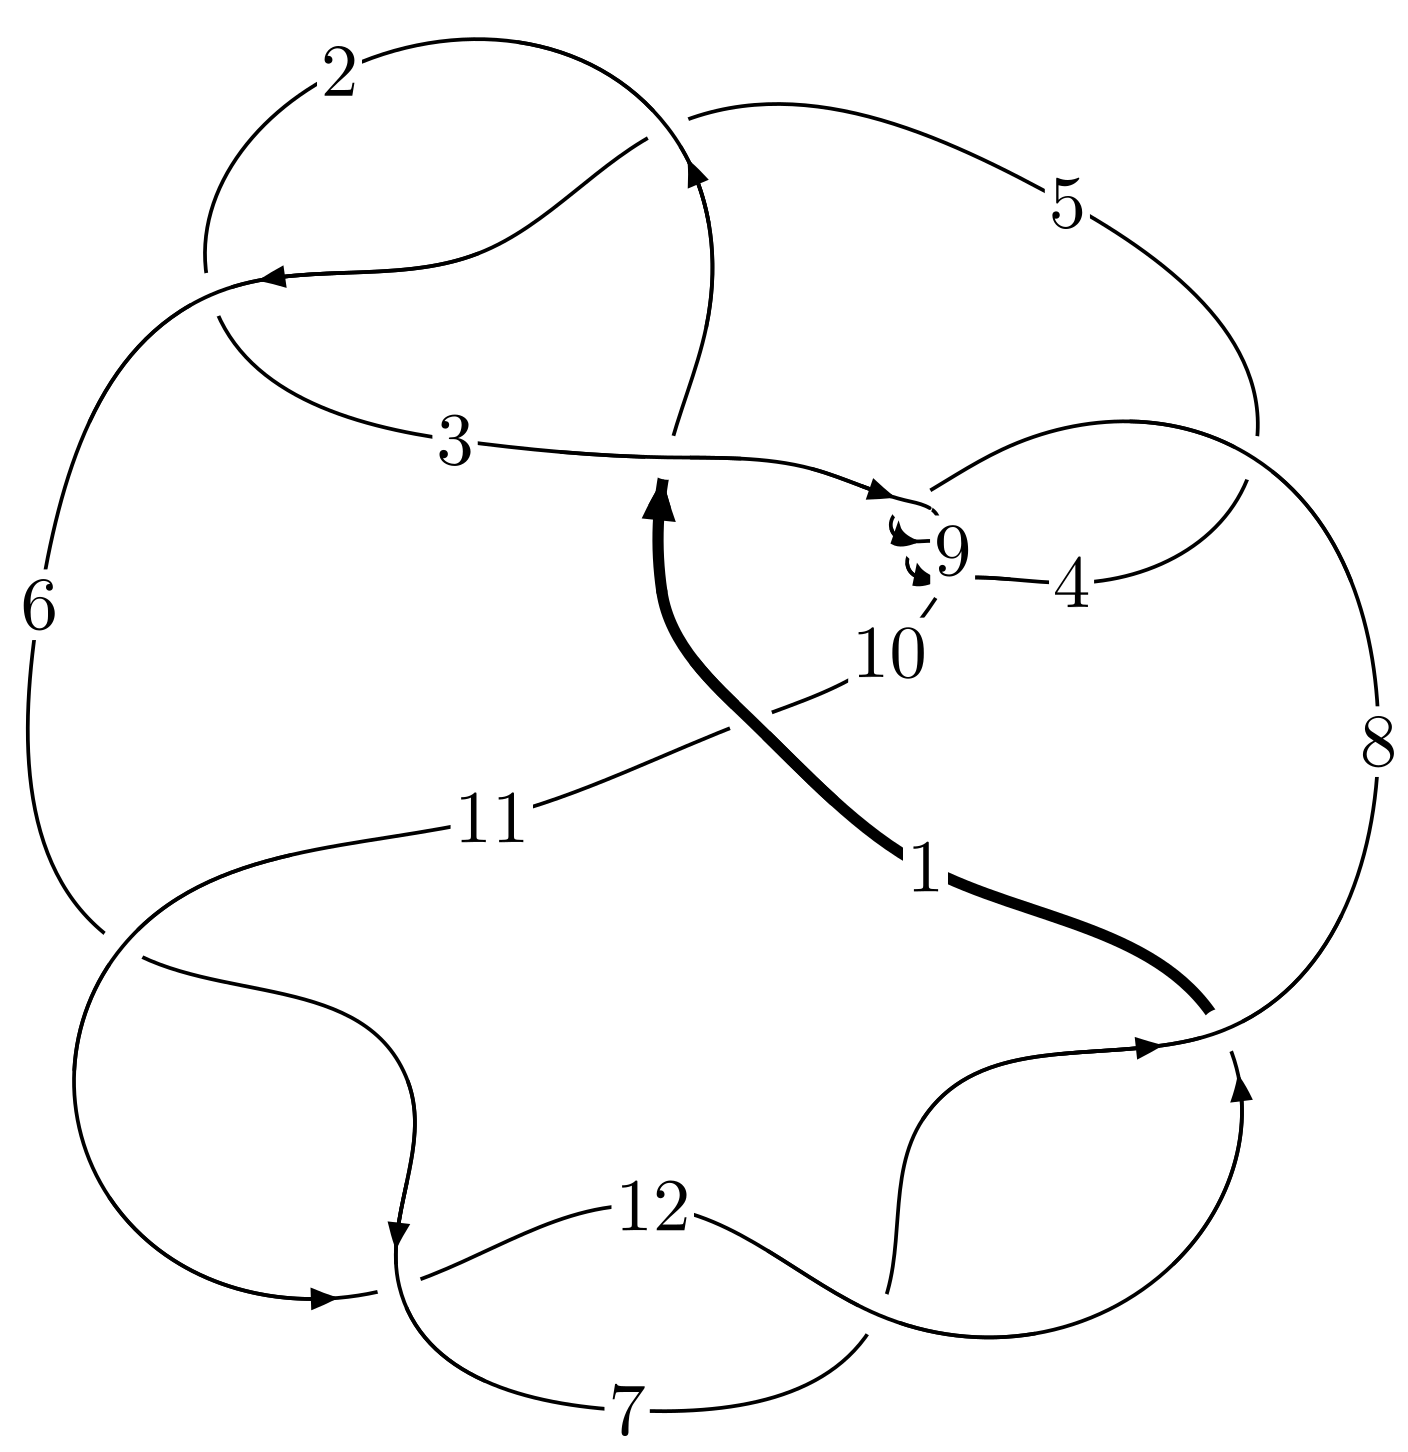
\includegraphics[width=112pt]{../../../GIT/diagram.site/Diagrams/png/2556_12n_0467.png}\\
\ \ \ A knot diagram\footnotemark}&
\allowdisplaybreaks
\textbf{Linearized knot diagam} \\
\cline{2-2}
 &
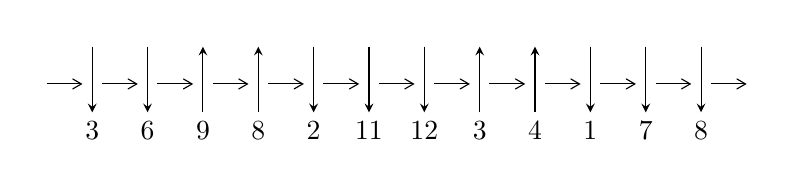
\begin{tikzpicture}[x=20pt, y=17pt]
	% nodes
	\node (C0) at (0, 0) {};
	\node (C1) at (1, 0) {};
	\node (C1U) at (1, +1) {};
	\node (C1D) at (1, -1) {3};

	\node (C2) at (2, 0) {};
	\node (C2U) at (2, +1) {};
	\node (C2D) at (2, -1) {6};

	\node (C3) at (3, 0) {};
	\node (C3U) at (3, +1) {};
	\node (C3D) at (3, -1) {9};

	\node (C4) at (4, 0) {};
	\node (C4U) at (4, +1) {};
	\node (C4D) at (4, -1) {8};

	\node (C5) at (5, 0) {};
	\node (C5U) at (5, +1) {};
	\node (C5D) at (5, -1) {2};

	\node (C6) at (6, 0) {};
	\node (C6U) at (6, +1) {};
	\node (C6D) at (6, -1) {11};

	\node (C7) at (7, 0) {};
	\node (C7U) at (7, +1) {};
	\node (C7D) at (7, -1) {12};

	\node (C8) at (8, 0) {};
	\node (C8U) at (8, +1) {};
	\node (C8D) at (8, -1) {3};

	\node (C9) at (9, 0) {};
	\node (C9U) at (9, +1) {};
	\node (C9D) at (9, -1) {4};

	\node (C10) at (10, 0) {};
	\node (C10U) at (10, +1) {};
	\node (C10D) at (10, -1) {1};

	\node (C11) at (11, 0) {};
	\node (C11U) at (11, +1) {};
	\node (C11D) at (11, -1) {7};

	\node (C12) at (12, 0) {};
	\node (C12U) at (12, +1) {};
	\node (C12D) at (12, -1) {8};
	\node (C13) at (13, 0) {};

	% arrows
	\draw[->,>={angle 60}]
	(C0) edge (C1) (C1) edge (C2) (C2) edge (C3) (C3) edge (C4) (C4) edge (C5) (C5) edge (C6) (C6) edge (C7) (C7) edge (C8) (C8) edge (C9) (C9) edge (C10) (C10) edge (C11) (C11) edge (C12) (C12) edge (C13) ;	\draw[->,>=stealth]
	(C1U) edge (C1D) (C2U) edge (C2D) (C3D) edge (C3U) (C4D) edge (C4U) (C5U) edge (C5D) (C6U) edge (C6D) (C7U) edge (C7D) (C8D) edge (C8U) (C9D) edge (C9U) (C10U) edge (C10D) (C11U) edge (C11D) (C12U) edge (C12D) ;
	\end{tikzpicture} \\
\hhline{~~} \\& 
\textbf{Solving Sequence} \\ \cline{2-2} 
 &
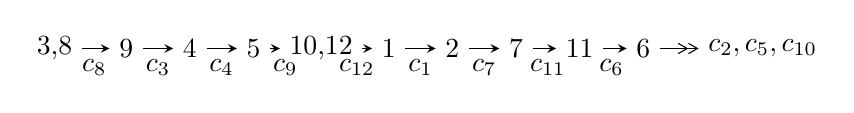
\begin{tikzpicture}[x=23pt, y=7pt]
	% node
	\node (A0) at (-1/8, 0) {3,8};
	\node (A1) at (1, 0) {9};
	\node (A2) at (2, 0) {4};
	\node (A3) at (3, 0) {5};
	\node (A4) at (65/16, 0) {10,12};
	\node (A5) at (41/8, 0) {1};
	\node (A6) at (49/8, 0) {2};
	\node (A7) at (57/8, 0) {7};
	\node (A8) at (65/8, 0) {11};
	\node (A9) at (73/8, 0) {6};
	\node (C1) at (1/2, -1) {$c_{8}$};
	\node (C2) at (3/2, -1) {$c_{3}$};
	\node (C3) at (5/2, -1) {$c_{4}$};
	\node (C4) at (7/2, -1) {$c_{9}$};
	\node (C5) at (37/8, -1) {$c_{12}$};
	\node (C6) at (45/8, -1) {$c_{1}$};
	\node (C7) at (53/8, -1) {$c_{7}$};
	\node (C8) at (61/8, -1) {$c_{11}$};
	\node (C9) at (69/8, -1) {$c_{6}$};
	\node (A10) at (11, 0) {$c_{2},c_{5},c_{10}$};

	% edge
	\draw[->,>=stealth]	
	(A0) edge (A1) (A1) edge (A2) (A2) edge (A3) (A3) edge (A4) (A4) edge (A5) (A5) edge (A6) (A6) edge (A7) (A7) edge (A8) (A8) edge (A9) ;
	\draw[->>,>={angle 60}]	
	(A9) edge (A10);
\end{tikzpicture} \\ 

\end{tabular} \\

\footnotetext{
The image of knot diagram is generated by the software ``\textbf{Draw programme}" developed by Andrew Bartholomew(\url{http://www.layer8.co.uk/maths/draw/index.htm\#Running-draw}), where we modified some parts for our purpose(\url{https://github.com/CATsTAILs/LinksPainter}).
}\phantom \\ \newline 
\centering \textbf{Ideals for irreducible components\footnotemark of $X_{\text{par}}$} 
 
\begin{align*}
I^u_{1}&=\langle 
140613342 u^{26}+233504827 u^{25}+\cdots+1306898116 b+2324027520,\\
\phantom{I^u_{1}}&\phantom{= \langle  }315767111 u^{26}+587740472 u^{25}+\cdots+1306898116 a-1648431188,\;u^{27}+u^{26}+\cdots-4 u-4\rangle \\
I^u_{2}&=\langle 
2 b-2 a+u,\;2 a^2-2 a u-2 a+u-1,\;u^2-2\rangle \\
\\
I^v_{1}&=\langle 
a,\;b+v+1,\;v^2+v-1\rangle \\
\end{align*}
\raggedright * 3 irreducible components of $\dim_{\mathbb{C}}=0$, with total 33 representations.\\
\footnotetext{All coefficients of polynomials are rational numbers. But the coefficients are sometimes approximated in decimal forms when there is not enough margin.}
\newpage
\renewcommand{\arraystretch}{1}
\centering \section*{I. $I^u_{1}= \langle 1.41\times10^{8} u^{26}+2.34\times10^{8} u^{25}+\cdots+1.31\times10^{9} b+2.32\times10^{9},\;3.16\times10^{8} u^{26}+5.88\times10^{8} u^{25}+\cdots+1.31\times10^{9} a-1.65\times10^{9},\;u^{27}+u^{26}+\cdots-4 u-4 \rangle$}
\flushleft \textbf{(i) Arc colorings}\\
\begin{tabular}{m{7pt} m{180pt} m{7pt} m{180pt} }
\flushright $a_{3}=$&$\begin{pmatrix}0\\u\end{pmatrix}$ \\
\flushright $a_{8}=$&$\begin{pmatrix}1\\0\end{pmatrix}$ \\
\flushright $a_{9}=$&$\begin{pmatrix}1\\- u^2\end{pmatrix}$ \\
\flushright $a_{4}=$&$\begin{pmatrix}u\\- u^3+u\end{pmatrix}$ \\
\flushright $a_{5}=$&$\begin{pmatrix}- u^3+2 u\\- u^3+u\end{pmatrix}$ \\
\flushright $a_{10}=$&$\begin{pmatrix}- u^2+1\\u^4-2 u^2\end{pmatrix}$ \\
\flushright $a_{12}=$&$\begin{pmatrix}-0.241616 u^{26}-0.449722 u^{25}+\cdots-13.1892 u+1.26133\\-0.107593 u^{26}-0.178671 u^{25}+\cdots-2.19364 u-1.77828\end{pmatrix}$ \\
\flushright $a_{1}=$&$\begin{pmatrix}-0.134023 u^{26}-0.271051 u^{25}+\cdots-10.9955 u+3.03961\\-0.107593 u^{26}-0.178671 u^{25}+\cdots-2.19364 u-1.77828\end{pmatrix}$ \\
\flushright $a_{2}=$&$\begin{pmatrix}-0.134023 u^{26}-0.271051 u^{25}+\cdots-10.9955 u+3.03961\\0.0945547 u^{26}-0.183568 u^{25}+\cdots-3.27784 u-2.32639\end{pmatrix}$ \\
\flushright $a_{7}=$&$\begin{pmatrix}-0.673320 u^{26}-0.574468 u^{25}+\cdots-15.4301 u+0.529920\\-0.102694 u^{26}+0.0537208 u^{25}+\cdots-3.65606 u-0.825481\end{pmatrix}$ \\
\flushright $a_{11}=$&$\begin{pmatrix}-0.00809889 u^{26}+0.000418223 u^{25}+\cdots+2.05151 u+3.50212\\0.355054 u^{26}+0.372385 u^{25}+\cdots+7.65668 u+1.09099\end{pmatrix}$ \\
\flushright $a_{6}=$&$\begin{pmatrix}-0.409090 u^{26}+0.0395121 u^{25}+\cdots-4.08989 u+7.12801\\-0.180513 u^{26}+0.126995 u^{25}+\cdots+3.62778 u+1.76201\end{pmatrix}$\\&\end{tabular}
\flushleft \textbf{(ii) Obstruction class $= -1$}\\~\\
\flushleft \textbf{(iii) Cusp Shapes $= -\frac{9879130}{326724529} u^{26}+\frac{101640265}{326724529} u^{25}+\cdots-\frac{4373584718}{326724529} u+\frac{3242559308}{326724529}$}\\~\\
\newpage\renewcommand{\arraystretch}{1}
\flushleft \textbf{(iv) u-Polynomials at the component}\newline \\
\begin{tabular}{m{50pt}|m{274pt}}
Crossings & \hspace{64pt}u-Polynomials at each crossing \\
\hline $$\begin{aligned}c_{1}\end{aligned}$$&$\begin{aligned}
&u^{27}+7 u^{26}+\cdots+73 u+1
\end{aligned}$\\
\hline $$\begin{aligned}c_{2},c_{5}\end{aligned}$$&$\begin{aligned}
&u^{27}+3 u^{26}+\cdots+7 u+1
\end{aligned}$\\
\hline $$\begin{aligned}c_{3},c_{8},c_{9}\end{aligned}$$&$\begin{aligned}
&u^{27}+u^{26}+\cdots-4 u-4
\end{aligned}$\\
\hline $$\begin{aligned}c_{4}\end{aligned}$$&$\begin{aligned}
&u^{27}-3 u^{26}+\cdots+612 u+220
\end{aligned}$\\
\hline $$\begin{aligned}c_{6},c_{7},c_{11}\\c_{12}\end{aligned}$$&$\begin{aligned}
&u^{27}-2 u^{26}+\cdots-6 u+1
\end{aligned}$\\
\hline $$\begin{aligned}c_{10}\end{aligned}$$&$\begin{aligned}
&u^{27}-2 u^{26}+\cdots-20 u-1
\end{aligned}$\\
\hline
\end{tabular}\\~\\
\newpage\renewcommand{\arraystretch}{1}
\flushleft \textbf{(v) Riley Polynomials at the component}\newline \\
\begin{tabular}{m{50pt}|m{274pt}}
Crossings & \hspace{64pt}Riley Polynomials at each crossing \\
\hline $$\begin{aligned}c_{1}\end{aligned}$$&$\begin{aligned}
&y^{27}+33 y^{26}+\cdots+4113 y-1
\end{aligned}$\\
\hline $$\begin{aligned}c_{2},c_{5}\end{aligned}$$&$\begin{aligned}
&y^{27}-7 y^{26}+\cdots+73 y-1
\end{aligned}$\\
\hline $$\begin{aligned}c_{3},c_{8},c_{9}\end{aligned}$$&$\begin{aligned}
&y^{27}-37 y^{26}+\cdots+336 y-16
\end{aligned}$\\
\hline $$\begin{aligned}c_{4}\end{aligned}$$&$\begin{aligned}
&y^{27}-97 y^{26}+\cdots+1370704 y-48400
\end{aligned}$\\
\hline $$\begin{aligned}c_{6},c_{7},c_{11}\\c_{12}\end{aligned}$$&$\begin{aligned}
&y^{27}-30 y^{26}+\cdots+32 y-1
\end{aligned}$\\
\hline $$\begin{aligned}c_{10}\end{aligned}$$&$\begin{aligned}
&y^{27}+42 y^{26}+\cdots+160 y-1
\end{aligned}$\\
\hline
\end{tabular}\\~\\
\newpage\flushleft \textbf{(vi) Complex Volumes and Cusp Shapes}
$$\begin{array}{c|c|c}  
\text{Solutions to }I^u_{1}& \I (\text{vol} + \sqrt{-1}CS) & \text{Cusp shape}\\
 \hline 
\begin{aligned}
u &= \phantom{-}0.910258 + 0.590456 I \\
a &= \phantom{-}2.00698 + 1.21820 I \\
b &= \phantom{-}1.50366 - 0.20859 I\end{aligned}
 & -3.25530 + 7.25549 I & -5.95539 - 6.08777 I \\ \hline\begin{aligned}
u &= \phantom{-}0.910258 - 0.590456 I \\
a &= \phantom{-}2.00698 - 1.21820 I \\
b &= \phantom{-}1.50366 + 0.20859 I\end{aligned}
 & -3.25530 - 7.25549 I & -5.95539 + 6.08777 I \\ \hline\begin{aligned}
u &= -1.017290 + 0.392893 I \\
a &= \phantom{-}1.59907 - 0.86702 I \\
b &= \phantom{-}1.384080 + 0.097780 I\end{aligned}
 & -2.42951 - 1.33319 I & -4.55270 + 1.10070 I \\ \hline\begin{aligned}
u &= -1.017290 - 0.392893 I \\
a &= \phantom{-}1.59907 + 0.86702 I \\
b &= \phantom{-}1.384080 - 0.097780 I\end{aligned}
 & -2.42951 + 1.33319 I & -4.55270 - 1.10070 I \\ \hline\begin{aligned}
u &= -1.028180 + 0.401751 I \\
a &= -0.842937 + 0.402129 I \\
b &= -0.466581 - 0.606665 I\end{aligned}
 & \phantom{-}3.20449 - 4.27323 I & -1.36721 + 6.77417 I \\ \hline\begin{aligned}
u &= -1.028180 - 0.401751 I \\
a &= -0.842937 - 0.402129 I \\
b &= -0.466581 + 0.606665 I\end{aligned}
 & \phantom{-}3.20449 + 4.27323 I & -1.36721 - 6.77417 I \\ \hline\begin{aligned}
u &= \phantom{-}1.132760 + 0.119465 I \\
a &= -0.399911 + 0.146187 I \\
b &= -0.444802 - 0.471118 I\end{aligned}
 & \phantom{-}3.11947 + 0.51181 I & -0.345493 + 0.472617 I \\ \hline\begin{aligned}
u &= \phantom{-}1.132760 - 0.119465 I \\
a &= -0.399911 - 0.146187 I \\
b &= -0.444802 + 0.471118 I\end{aligned}
 & \phantom{-}3.11947 - 0.51181 I & -0.345493 - 0.472617 I \\ \hline\begin{aligned}
u &= \phantom{-}0.068539 + 0.776104 I \\
a &= -2.94508 - 0.05064 I \\
b &= -1.42888 - 0.10362 I\end{aligned}
 & -5.79751 - 2.66305 I & -8.58849 + 2.68063 I \\ \hline\begin{aligned}
u &= \phantom{-}0.068539 - 0.776104 I \\
a &= -2.94508 + 0.05064 I \\
b &= -1.42888 + 0.10362 I\end{aligned}
 & -5.79751 + 2.66305 I & -8.58849 - 2.68063 I\\
 \hline 
 \end{array}$$\newpage$$\begin{array}{c|c|c}  
\text{Solutions to }I^u_{1}& \I (\text{vol} + \sqrt{-1}CS) & \text{Cusp shape}\\
 \hline 
\begin{aligned}
u &= \phantom{-}0.701128\phantom{ +0.000000I} \\
a &= -0.723697\phantom{ +0.000000I} \\
b &= \phantom{-}1.54174\phantom{ +0.000000I}\end{aligned}
 & -9.07206\phantom{ +0.000000I} & -6.92100\phantom{ +0.000000I} \\ \hline\begin{aligned}
u &= \phantom{-}1.38081\phantom{ +0.000000I} \\
a &= -0.782809\phantom{ +0.000000I} \\
b &= -0.202634\phantom{ +0.000000I}\end{aligned}
 & \phantom{-}3.22160\phantom{ +0.000000I} & \phantom{-}2.65910\phantom{ +0.000000I} \\ \hline\begin{aligned}
u &= -1.43515\phantom{ +0.000000I} \\
a &= \phantom{-}1.63913\phantom{ +0.000000I} \\
b &= \phantom{-}1.62828\phantom{ +0.000000I}\end{aligned}
 & -3.96458\phantom{ +0.000000I} & -1.96340\phantom{ +0.000000I} \\ \hline\begin{aligned}
u &= \phantom{-}0.093206 + 0.505933 I \\
a &= \phantom{-}0.909549 - 0.188312 I \\
b &= \phantom{-}0.279075 - 0.365424 I\end{aligned}
 & -0.272367 + 1.017390 I & -4.41879 - 6.56996 I \\ \hline\begin{aligned}
u &= \phantom{-}0.093206 - 0.505933 I \\
a &= \phantom{-}0.909549 + 0.188312 I \\
b &= \phantom{-}0.279075 + 0.365424 I\end{aligned}
 & -0.272367 - 1.017390 I & -4.41879 + 6.56996 I \\ \hline\begin{aligned}
u &= -0.462517\phantom{ +0.000000I} \\
a &= \phantom{-}1.41263\phantom{ +0.000000I} \\
b &= \phantom{-}0.790251\phantom{ +0.000000I}\end{aligned}
 & -1.60060\phantom{ +0.000000I} & -3.53340\phantom{ +0.000000I} \\ \hline\begin{aligned}
u &= -1.60836\phantom{ +0.000000I} \\
a &= -0.0902962\phantom{ +0.000000I} \\
b &= -1.36994\phantom{ +0.000000I}\end{aligned}
 & -1.00091\phantom{ +0.000000I} & -6.04390\phantom{ +0.000000I} \\ \hline\begin{aligned}
u &= \phantom{-}0.389158\phantom{ +0.000000I} \\
a &= -3.32064\phantom{ +0.000000I} \\
b &= -1.64070\phantom{ +0.000000I}\end{aligned}
 & -10.0949\phantom{ +0.000000I} & \phantom{-}1.45710\phantom{ +0.000000I} \\ \hline\begin{aligned}
u &= -0.327289\phantom{ +0.000000I} \\
a &= \phantom{-}3.18758\phantom{ +0.000000I} \\
b &= -0.436653\phantom{ +0.000000I}\end{aligned}
 & -2.27386\phantom{ +0.000000I} & \phantom{-}5.71450\phantom{ +0.000000I} \\ \hline\begin{aligned}
u &= -1.70507 + 0.18041 I \\
a &= -1.29573 + 0.99047 I \\
b &= -1.58969 - 0.26870 I\end{aligned}
 & \phantom{-}5.77830 - 10.34990 I & -4.51654 + 4.83744 I\\
 \hline 
 \end{array}$$\newpage$$\begin{array}{c|c|c}  
\text{Solutions to }I^u_{1}& \I (\text{vol} + \sqrt{-1}CS) & \text{Cusp shape}\\
 \hline 
\begin{aligned}
u &= -1.70507 - 0.18041 I \\
a &= -1.29573 - 0.99047 I \\
b &= -1.58969 + 0.26870 I\end{aligned}
 & \phantom{-}5.77830 + 10.34990 I & -4.51654 - 4.83744 I \\ \hline\begin{aligned}
u &= \phantom{-}1.74296 + 0.07415 I \\
a &= -1.029860 - 0.595198 I \\
b &= -1.47829 + 0.32375 I\end{aligned}
 & \phantom{-}7.48038 + 3.07161 I & -3.06454 - 1.05246 I \\ \hline\begin{aligned}
u &= \phantom{-}1.74296 - 0.07415 I \\
a &= -1.029860 + 0.595198 I \\
b &= -1.47829 - 0.32375 I\end{aligned}
 & \phantom{-}7.48038 - 3.07161 I & -3.06454 + 1.05246 I \\ \hline\begin{aligned}
u &= \phantom{-}1.74801 + 0.11240 I \\
a &= \phantom{-}0.591464 + 0.471611 I \\
b &= \phantom{-}0.634607 - 0.775759 I\end{aligned}
 & \phantom{-}13.1108 + 6.4432 I & -1.45116 - 4.64591 I \\ \hline\begin{aligned}
u &= \phantom{-}1.74801 - 0.11240 I \\
a &= \phantom{-}0.591464 - 0.471611 I \\
b &= \phantom{-}0.634607 + 0.775759 I\end{aligned}
 & \phantom{-}13.1108 - 6.4432 I & -1.45116 + 4.64591 I \\ \hline\begin{aligned}
u &= -1.76409 + 0.02868 I \\
a &= \phantom{-}0.245519 + 0.313706 I \\
b &= \phantom{-}0.451661 - 0.831495 I\end{aligned}
 & \phantom{-}13.66050 - 1.13182 I & -0.424228 - 0.165787 I \\ \hline\begin{aligned}
u &= -1.76409 - 0.02868 I \\
a &= \phantom{-}0.245519 - 0.313706 I \\
b &= \phantom{-}0.451661 + 0.831495 I\end{aligned}
 & \phantom{-}13.66050 + 1.13182 I & -0.424228 + 0.165787 I\\
 \hline 
 \end{array}$$\newpage\newpage\renewcommand{\arraystretch}{1}
\centering \section*{II. $I^u_{2}= \langle 2 b-2 a+u,\;2 a^2-2 a u-2 a+u-1,\;u^2-2 \rangle$}
\flushleft \textbf{(i) Arc colorings}\\
\begin{tabular}{m{7pt} m{180pt} m{7pt} m{180pt} }
\flushright $a_{3}=$&$\begin{pmatrix}0\\u\end{pmatrix}$ \\
\flushright $a_{8}=$&$\begin{pmatrix}1\\0\end{pmatrix}$ \\
\flushright $a_{9}=$&$\begin{pmatrix}1\\-2\end{pmatrix}$ \\
\flushright $a_{4}=$&$\begin{pmatrix}u\\- u\end{pmatrix}$ \\
\flushright $a_{5}=$&$\begin{pmatrix}0\\- u\end{pmatrix}$ \\
\flushright $a_{10}=$&$\begin{pmatrix}-1\\0\end{pmatrix}$ \\
\flushright $a_{12}=$&$\begin{pmatrix}a\\a-\frac{1}{2} u\end{pmatrix}$ \\
\flushright $a_{1}=$&$\begin{pmatrix}\frac{1}{2} u\\a-\frac{1}{2} u\end{pmatrix}$ \\
\flushright $a_{2}=$&$\begin{pmatrix}\frac{1}{2} u\\a+\frac{1}{2} u\end{pmatrix}$ \\
\flushright $a_{7}=$&$\begin{pmatrix}-\frac{1}{2} a u- a+\frac{1}{2} u+\frac{1}{2}\\- a+\frac{1}{2} u-1\end{pmatrix}$ \\
\flushright $a_{11}=$&$\begin{pmatrix}-\frac{1}{2} a u-\frac{1}{2}\\- a+\frac{1}{2} u-1\end{pmatrix}$ \\
\flushright $a_{6}=$&$\begin{pmatrix}\frac{1}{2} u\\a-\frac{1}{2} u\end{pmatrix}$\\&\end{tabular}
\flushleft \textbf{(ii) Obstruction class $= 1$}\\~\\
\flushleft \textbf{(iii) Cusp Shapes $= -8$}\\~\\
\newpage\renewcommand{\arraystretch}{1}
\flushleft \textbf{(iv) u-Polynomials at the component}\newline \\
\begin{tabular}{m{50pt}|m{274pt}}
Crossings & \hspace{64pt}u-Polynomials at each crossing \\
\hline $$\begin{aligned}c_{1},c_{5}\end{aligned}$$&$\begin{aligned}
&(u-1)^4
\end{aligned}$\\
\hline $$\begin{aligned}c_{2}\end{aligned}$$&$\begin{aligned}
&(u+1)^4
\end{aligned}$\\
\hline $$\begin{aligned}c_{3},c_{4},c_{8}\\c_{9}\end{aligned}$$&$\begin{aligned}
&(u^2-2)^2
\end{aligned}$\\
\hline $$\begin{aligned}c_{6},c_{7}\end{aligned}$$&$\begin{aligned}
&(u^2- u-1)^2
\end{aligned}$\\
\hline $$\begin{aligned}c_{10},c_{11},c_{12}\end{aligned}$$&$\begin{aligned}
&(u^2+u-1)^2
\end{aligned}$\\
\hline
\end{tabular}\\~\\
\newpage\renewcommand{\arraystretch}{1}
\flushleft \textbf{(v) Riley Polynomials at the component}\newline \\
\begin{tabular}{m{50pt}|m{274pt}}
Crossings & \hspace{64pt}Riley Polynomials at each crossing \\
\hline $$\begin{aligned}c_{1},c_{2},c_{5}\end{aligned}$$&$\begin{aligned}
&(y-1)^4
\end{aligned}$\\
\hline $$\begin{aligned}c_{3},c_{4},c_{8}\\c_{9}\end{aligned}$$&$\begin{aligned}
&(y-2)^4
\end{aligned}$\\
\hline $$\begin{aligned}c_{6},c_{7},c_{10}\\c_{11},c_{12}\end{aligned}$$&$\begin{aligned}
&(y^2-3 y+1)^2
\end{aligned}$\\
\hline
\end{tabular}\\~\\
\newpage\flushleft \textbf{(vi) Complex Volumes and Cusp Shapes}
$$\begin{array}{c|c|c}  
\text{Solutions to }I^u_{2}& \I (\text{vol} + \sqrt{-1}CS) & \text{Cusp shape}\\
 \hline 
\begin{aligned}
u &= \phantom{-}1.41421\phantom{ +0.000000I} \\
a &= \phantom{-}0.0890728\phantom{ +0.000000I} \\
b &= -0.618034\phantom{ +0.000000I}\end{aligned}
 & \phantom{-}2.30291\phantom{ +0.000000I} & -8.00000\phantom{ +0.000000I} \\ \hline\begin{aligned}
u &= \phantom{-}1.41421\phantom{ +0.000000I} \\
a &= \phantom{-}2.32514\phantom{ +0.000000I} \\
b &= \phantom{-}1.61803\phantom{ +0.000000I}\end{aligned}
 & -5.59278\phantom{ +0.000000I} & -8.00000\phantom{ +0.000000I} \\ \hline\begin{aligned}
u &= -1.41421\phantom{ +0.000000I} \\
a &= \phantom{-}0.910927\phantom{ +0.000000I} \\
b &= \phantom{-}1.61803\phantom{ +0.000000I}\end{aligned}
 & -5.59278\phantom{ +0.000000I} & -8.00000\phantom{ +0.000000I} \\ \hline\begin{aligned}
u &= -1.41421\phantom{ +0.000000I} \\
a &= -1.32514\phantom{ +0.000000I} \\
b &= -0.618034\phantom{ +0.000000I}\end{aligned}
 & \phantom{-}2.30291\phantom{ +0.000000I} & -8.00000\phantom{ +0.000000I}\\
 \hline 
 \end{array}$$\newpage\newpage\renewcommand{\arraystretch}{1}
\centering \section*{III. $I^v_{1}= \langle a,\;b+v+1,\;v^2+v-1 \rangle$}
\flushleft \textbf{(i) Arc colorings}\\
\begin{tabular}{m{7pt} m{180pt} m{7pt} m{180pt} }
\flushright $a_{3}=$&$\begin{pmatrix}v\\0\end{pmatrix}$ \\
\flushright $a_{8}=$&$\begin{pmatrix}1\\0\end{pmatrix}$ \\
\flushright $a_{9}=$&$\begin{pmatrix}1\\0\end{pmatrix}$ \\
\flushright $a_{4}=$&$\begin{pmatrix}v\\0\end{pmatrix}$ \\
\flushright $a_{5}=$&$\begin{pmatrix}v\\0\end{pmatrix}$ \\
\flushright $a_{10}=$&$\begin{pmatrix}1\\0\end{pmatrix}$ \\
\flushright $a_{12}=$&$\begin{pmatrix}0\\- v-1\end{pmatrix}$ \\
\flushright $a_{1}=$&$\begin{pmatrix}v+1\\- v-1\end{pmatrix}$ \\
\flushright $a_{2}=$&$\begin{pmatrix}2 v+1\\- v-1\end{pmatrix}$ \\
\flushright $a_{7}=$&$\begin{pmatrix}1\\- v-2\end{pmatrix}$ \\
\flushright $a_{11}=$&$\begin{pmatrix}- v-1\\v+2\end{pmatrix}$ \\
\flushright $a_{6}=$&$\begin{pmatrix}- v-1\\v+1\end{pmatrix}$\\&\end{tabular}
\flushleft \textbf{(ii) Obstruction class $= 1$}\\~\\
\flushleft \textbf{(iii) Cusp Shapes $= -18$}\\~\\
\newpage\renewcommand{\arraystretch}{1}
\flushleft \textbf{(iv) u-Polynomials at the component}\newline \\
\begin{tabular}{m{50pt}|m{274pt}}
Crossings & \hspace{64pt}u-Polynomials at each crossing \\
\hline $$\begin{aligned}c_{1},c_{2}\end{aligned}$$&$\begin{aligned}
&(u-1)^2
\end{aligned}$\\
\hline $$\begin{aligned}c_{3},c_{4},c_{8}\\c_{9}\end{aligned}$$&$\begin{aligned}
&u^2
\end{aligned}$\\
\hline $$\begin{aligned}c_{5}\end{aligned}$$&$\begin{aligned}
&(u+1)^2
\end{aligned}$\\
\hline $$\begin{aligned}c_{6},c_{7},c_{10}\end{aligned}$$&$\begin{aligned}
&u^2+u-1
\end{aligned}$\\
\hline $$\begin{aligned}c_{11},c_{12}\end{aligned}$$&$\begin{aligned}
&u^2- u-1
\end{aligned}$\\
\hline
\end{tabular}\\~\\
\newpage\renewcommand{\arraystretch}{1}
\flushleft \textbf{(v) Riley Polynomials at the component}\newline \\
\begin{tabular}{m{50pt}|m{274pt}}
Crossings & \hspace{64pt}Riley Polynomials at each crossing \\
\hline $$\begin{aligned}c_{1},c_{2},c_{5}\end{aligned}$$&$\begin{aligned}
&(y-1)^2
\end{aligned}$\\
\hline $$\begin{aligned}c_{3},c_{4},c_{8}\\c_{9}\end{aligned}$$&$\begin{aligned}
&y^2
\end{aligned}$\\
\hline $$\begin{aligned}c_{6},c_{7},c_{10}\\c_{11},c_{12}\end{aligned}$$&$\begin{aligned}
&y^2-3 y+1
\end{aligned}$\\
\hline
\end{tabular}\\~\\
\newpage\flushleft \textbf{(vi) Complex Volumes and Cusp Shapes}
$$\begin{array}{c|c|c}  
\text{Solutions to }I^v_{1}& \I (\text{vol} + \sqrt{-1}CS) & \text{Cusp shape}\\
 \hline 
\begin{aligned}
v &= \phantom{-}0.618034\phantom{ +0.000000I} \\
a &= \phantom{-0.000000 } 0 \\
b &= -1.61803\phantom{ +0.000000I}\end{aligned}
 & -10.5276\phantom{ +0.000000I} & -18.0000\phantom{ +0.000000I} \\ \hline\begin{aligned}
v &= -1.61803\phantom{ +0.000000I} \\
a &= \phantom{-0.000000 } 0 \\
b &= \phantom{-}0.618034\phantom{ +0.000000I}\end{aligned}
 & -2.63189\phantom{ +0.000000I} & -18.0000\phantom{ +0.000000I}\\
 \hline 
 \end{array}$$\newpage
\newpage\renewcommand{\arraystretch}{1}
\centering \section*{ IV. u-Polynomials}
\begin{tabular}{m{50pt}|m{274pt}}
Crossings & \hspace{64pt}u-Polynomials at each crossing \\
\hline $$\begin{aligned}c_{1}\end{aligned}$$&$\begin{aligned}
&((u-1)^6)(u^{27}+7 u^{26}+\cdots+73 u+1)
\end{aligned}$\\
\hline $$\begin{aligned}c_{2}\end{aligned}$$&$\begin{aligned}
&((u-1)^2)(u+1)^4(u^{27}+3 u^{26}+\cdots+7 u+1)
\end{aligned}$\\
\hline $$\begin{aligned}c_{3},c_{8},c_{9}\end{aligned}$$&$\begin{aligned}
&u^2(u^2-2)^2(u^{27}+u^{26}+\cdots-4 u-4)
\end{aligned}$\\
\hline $$\begin{aligned}c_{4}\end{aligned}$$&$\begin{aligned}
&u^2(u^2-2)^2(u^{27}-3 u^{26}+\cdots+612 u+220)
\end{aligned}$\\
\hline $$\begin{aligned}c_{5}\end{aligned}$$&$\begin{aligned}
&((u-1)^4)(u+1)^2(u^{27}+3 u^{26}+\cdots+7 u+1)
\end{aligned}$\\
\hline $$\begin{aligned}c_{6},c_{7}\end{aligned}$$&$\begin{aligned}
&((u^2- u-1)^2)(u^2+u-1)(u^{27}-2 u^{26}+\cdots-6 u+1)
\end{aligned}$\\
\hline $$\begin{aligned}c_{10}\end{aligned}$$&$\begin{aligned}
&((u^2+u-1)^3)(u^{27}-2 u^{26}+\cdots-20 u-1)
\end{aligned}$\\
\hline $$\begin{aligned}c_{11},c_{12}\end{aligned}$$&$\begin{aligned}
&(u^2- u-1)(u^2+u-1)^2(u^{27}-2 u^{26}+\cdots-6 u+1)
\end{aligned}$\\
\hline
\end{tabular}\newpage\renewcommand{\arraystretch}{1}
\centering \section*{ V. Riley Polynomials}
\begin{tabular}{m{50pt}|m{274pt}}
Crossings & \hspace{64pt}Riley Polynomials at each crossing \\
\hline $$\begin{aligned}c_{1}\end{aligned}$$&$\begin{aligned}
&((y-1)^6)(y^{27}+33 y^{26}+\cdots+4113 y-1)
\end{aligned}$\\
\hline $$\begin{aligned}c_{2},c_{5}\end{aligned}$$&$\begin{aligned}
&((y-1)^6)(y^{27}-7 y^{26}+\cdots+73 y-1)
\end{aligned}$\\
\hline $$\begin{aligned}c_{3},c_{8},c_{9}\end{aligned}$$&$\begin{aligned}
&y^2(y-2)^4(y^{27}-37 y^{26}+\cdots+336 y-16)
\end{aligned}$\\
\hline $$\begin{aligned}c_{4}\end{aligned}$$&$\begin{aligned}
&y^2(y-2)^4(y^{27}-97 y^{26}+\cdots+1370704 y-48400)
\end{aligned}$\\
\hline $$\begin{aligned}c_{6},c_{7},c_{11}\\c_{12}\end{aligned}$$&$\begin{aligned}
&((y^2-3 y+1)^3)(y^{27}-30 y^{26}+\cdots+32 y-1)
\end{aligned}$\\
\hline $$\begin{aligned}c_{10}\end{aligned}$$&$\begin{aligned}
&((y^2-3 y+1)^3)(y^{27}+42 y^{26}+\cdots+160 y-1)
\end{aligned}$\\
\hline
\end{tabular}
\vskip 2pc
\end{document}